\subsubsection{09.12.14}

\begin{enumerate}
	\item Время начала и окончания собрания:
	15:50 - 20:30
	\item Цели собрания:
	\begin{enumerate}
	  \item Укрепить ковш суперклеем.
	  
	  \item Протестировать, как механизм опрокидывания ковша справляется с новым ковшом.
	  
    \end{enumerate}
	\item Проделанная работа:
	\begin{enumerate}
	  \item Швы ковша были проклеены суперклеем.
	  
	  \item В процессе испытаний механизма опрокидывания ковша выяснилось, что сервоприводу не хватает мощности для того, чтобы поднимать ковш (поскольку теперь длина плеча ковша - 40 см, а установить полноценный противовес с противоположной стороны невозможно, так как механизм опрокидывания ковша находится в 1 см то верхней границы предельно допустимых габаритов робота). Пока мы не знаем, как решить эту проблему, но к следующему занятию мы постараемся придумать и на нем обсудить наши варианты решения проблемы.
	  
	  \item Сегодня у нас появилась стальная ось диаметром 8 мм и мы начали работать над заменой алюминиевых перекладин подъемника на стальные. На данный момент мы смогли только распилить ось на куски нужной длины, но на следующем занятии мы планируем закрепить их на роботе.
	  
	  \item Для того, чтобы закреплять оси, было решено просверлить в них отверстия и затем вставить в них винты с таким образом, что они не позволят оси выходить из пазов.
	  
	  \begin{figure}[H]
	  	\begin{minipage}[h]{0.2\linewidth}
	  		\center  
	  	\end{minipage}
	  	\begin{minipage}[h]{0.6\linewidth}
	  		\center{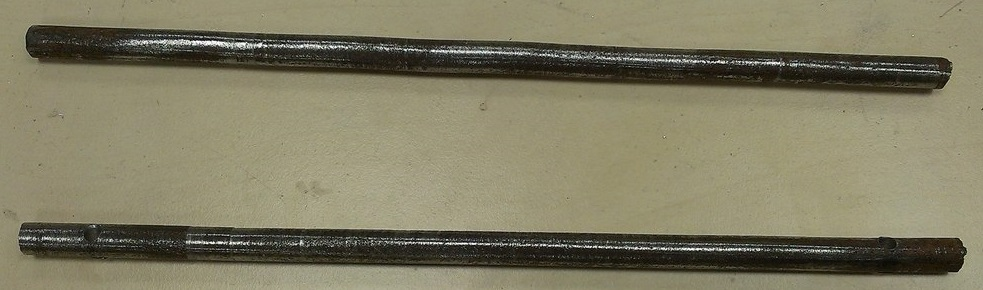
\includegraphics[scale=0.3]{days/09.12.14/images/01}}
	  		\caption{Ось распилена}
	  	\end{minipage}
	  \end{figure}
      
    \end{enumerate}
    
	\item Итоги собрания: 
	\begin{enumerate}
	  \item Ковш проклеен суперклеем.
	  
	  \item Механизм опрокидывания ковша испытан. На данный момен опрокидывание ковша невозможно.
	  
	  \item Стальная ось распилена на куски нужной длины.
	  
    \end{enumerate}
    
	\item Задачи для последующих собраний:
	\begin{enumerate}
	  \item Закрепить перекладины на подъемнике.
	  
	  \item Предложить идеи для решения проблемы с невозможностью опрокидывать ковш ковша.
	  
    \end{enumerate}     
\end{enumerate}
\fillpage